\documentclass[a4paper,12pt]{article}
\usepackage[utf8]{inputenc}
\usepackage[IL2]{fontenc}
\usepackage{listings}
\usepackage{amssymb}
\usepackage{amsmath}
\usepackage{url}
\usepackage{graphicx}
\usepackage[czech]{babel}
\usepackage[final]{pdfpages}
\title{MF004 -- semestrální projekt}
\author{Marek Bryša, 323771}
\date{Brno, \today}
\begin{document}
\maketitle
\section{Data}
  \subsection{Úvod}
    Zdrojem dat je soubor \texttt{MortgageDefaulters.xls}. Obsahuje údaje o 15153 klientech banky, kteří mají hypoteční úvěr. Cílem je identifikovat klienty s vysokou pravděpodobností, že nebudou splácet. K dispozici jsou tyto proměnné:
    \begin{description}
      \item[Bo\_Age] Věk klienta
      \item[Ln\_Orig] Výše půjčký v USD
      \item[Orig\_LTV\_Ratio\_Pct] Poměr půjcky a nákupní ceny domu
      \item[Credit\_score] Klientovo credit score
      \item[First\_home] První klientův nákup dům (Y/N)
      \item[Tot\_mthly\_debt\_exp] Klientův celkový měsíční výdaj na půjčku
      \item[Tot\_mthly\_incm] Klinetův celkový měsíční příjem
      \item[orig\_apprd\_val\_amt] Odhad ceny domu v době žádosti
      \item[pur\_prc\_amt] Kupní cena domu
      \item[DTI\_ratio] Poměr nákladu na dluh a příjmu klienta -- měsíčně 
      \item[StatusCurrent] Stav půjčky
      \item[OUTCOME] Binary binární verze stavu: 0=v pořádku, 1=default
      \item[StateUS] Stát USA, kde se dům nachází
      \item[Median\_state\_inc] Střední příjem domácnosti v daném státě (2002-2004)
      \item[UPB$>$Appraisal] Je půjčka vyšší než odhad? 0=ne, 1=ano
    \end{description}
  \subsection{Popisné statistiky}
    V následujíci tabulce jsou uvedeny popisné statistiky intervalových proměnných:
    \begin{center}
    \begin{tabular}{|l|r|r|r|r|r|r|r|r|r|r|}
      \hline
      %%%%%%%%%%%%%%%%%%%%%%%%%%%%%%%%%%%%%%%%%%%%%%%%%%%%%%%%%%%%%%%%%%%%%%
%%                                                                  %%
%%  This is a LaTeX2e table fragment exported from Gnumeric.        %%
%%                                                                  %%
%%%%%%%%%%%%%%%%%%%%%%%%%%%%%%%%%%%%%%%%%%%%%%%%%%%%%%%%%%%%%%%%%%%%%%
	&Mean	&Std.Err.	&Median	&Std.Dev.	&Min	&Max\\\hline
Bo\_Age	&36.79	&0.08	&37	&10.03	&18	&99\\\hline
Ln\_Orig	&153467.57	&555.42	&141500	&68370.61	&19600	&599000\\\hline
Orig\_LTV\_Ratio\_Pct	&93.08	&0.07	&95	&8.85	&20	&111\\\hline
Credit\_score	&687.67	&0.51	&688	&62.90	&440	&999\\\hline
Tot\_mthly\_debt\_exp	&1745.46	&8.85	&1578	&1089.20	&0	&17225\\\hline
Tot\_mthly\_incm	&5024.71	&23.98	&4632	&2952.16	&500	&65000\\\hline
orig\_apprd\_val\_amt	&170661.44	&664.31	&154000	&81775.07	&0	&870000\\\hline
pur\_prc\_amt	&164681.56	&647.62	&148650	&79719.84	&20000	&870000\\\hline
DTI Ratio	&0.37	&0.00	&0	&0.18	&0	&3\\\hline
Median\_state\_inc	&44945.07	&44.12	&43988	&5431.51	&32589	&57352\\\hline

    \end{tabular}
    \end{center}
    Je zřejmé, že data obsahují některé podezřelé hodnoty. Bude nunté porvést transformaci.
  \subsection{Transformace dat}
    U 903 klientů je proměnná \texttt{Tot\_mthly\_debt\_exp} nulová. Tím je u stejného počtu nulová i proměnná \texttt{DTI\_Ratio}. U ostatních klientů nabývá \texttt{Tot\_mthly\_debt\_exp} v průměru 0.016045 násobku \texttt{Ln\_Orig}. Touto hodnotou nulu nahradíme a dopočteme \texttt{DTI\_Ratio}.
    
    U 19 klientů je \texttt{orig\_apprd\_val\_amt} nulová. Stejným postupem ji rekonstruujeme z \texttt{pur\_prc\_amt}, přičemž u ostatních klientů platí, že \[
    \texttt{orig\_apprd\_val\_amt} =  1.059314\cdot \texttt{pur\_prc\_amt}.
\]

	Dále budeme pracovat s daty kategorizovanými podle decilů.
  \section{Regrese}
	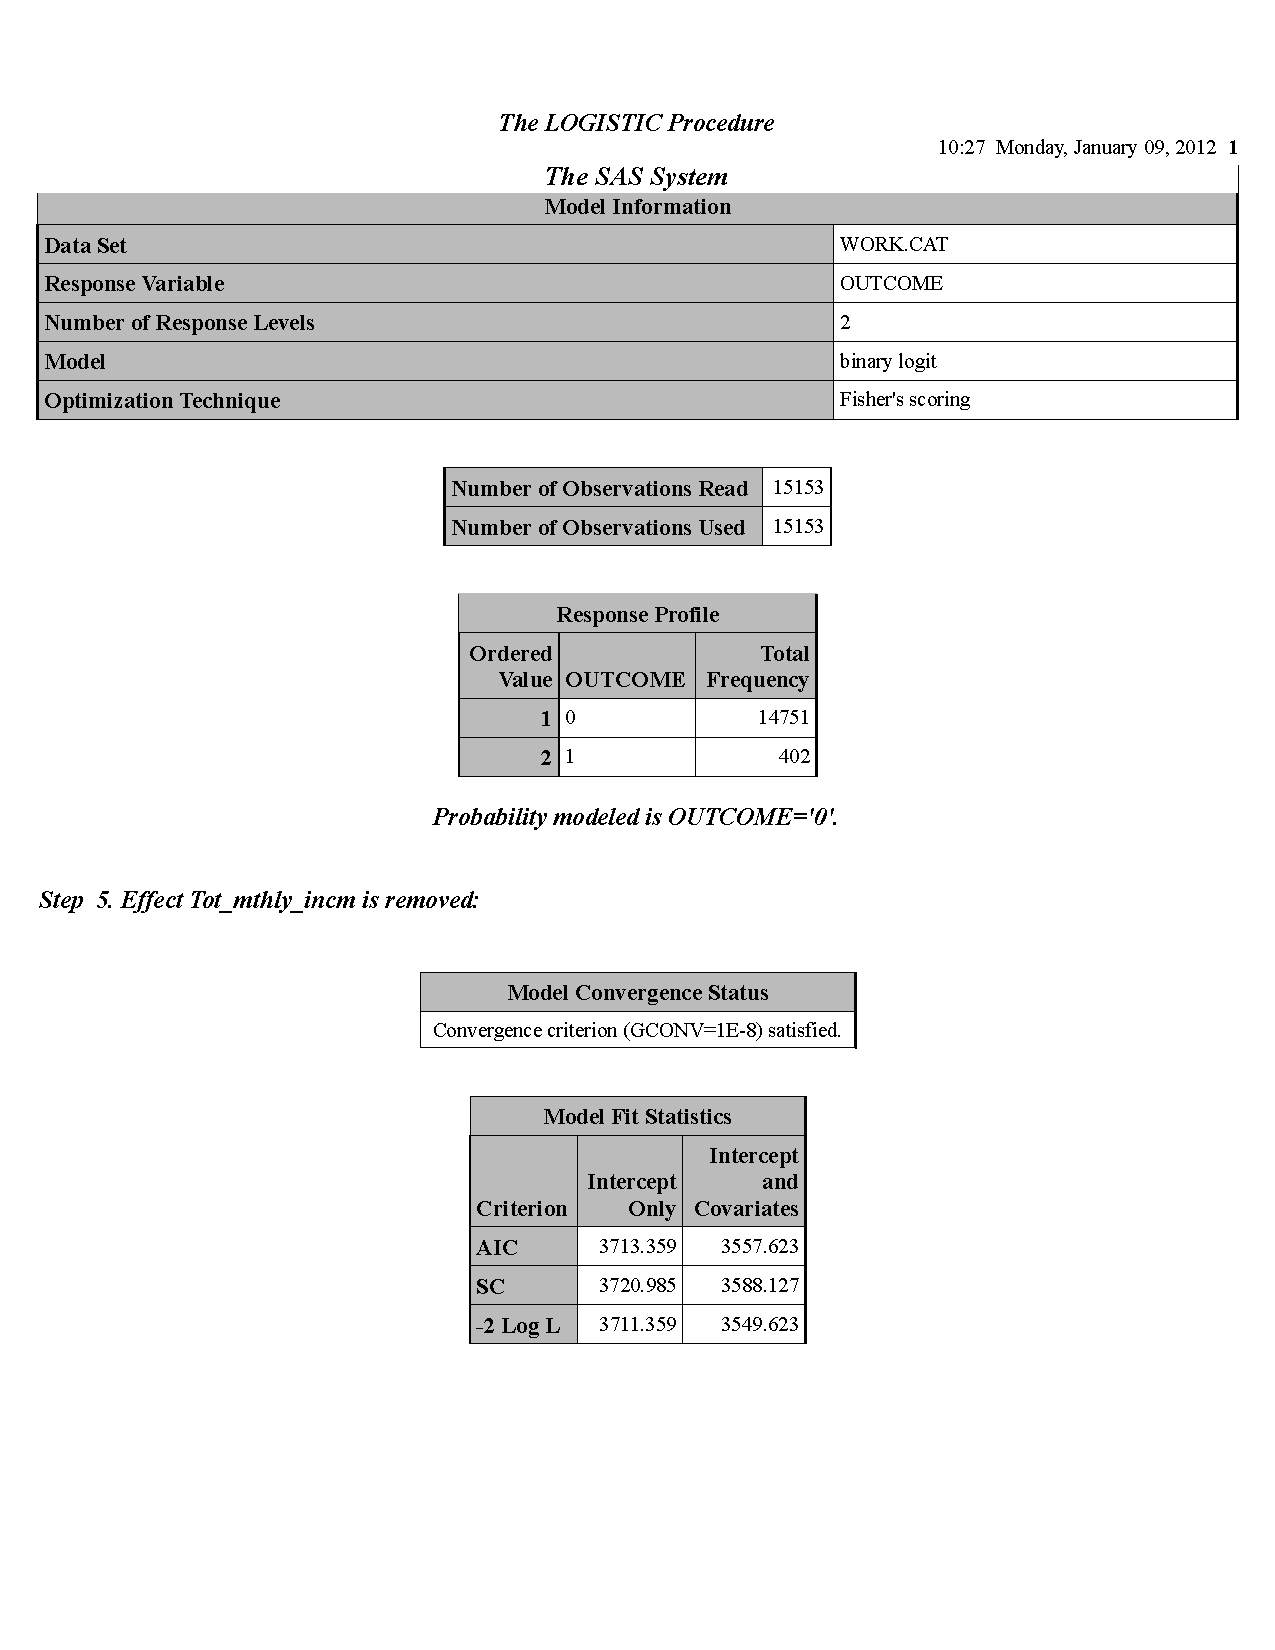
\includepdf[pages={1,2,3}]{logitshort.pdf}
	Byla použita metoda stepwise, která přidáva a odebíra vysvětlující proměnné podle jejich statistické významnosti. Výsledkem je model se třemi proměnnými. Hypotézu o celkové nevýznamnosti modelu zamítáme. 
	
	Pokud klient žádá o půjčku na svůj první dům, snižuje se šance nesplácení. Stejně tak má pozitivní vliv credit score přidělené při žádosti o úvěr. Dále platí, že klient je tím lepší, čím vyšší jsou jeho měsíční výdaje na splátky dluhu. To lze vystvětlit tím, že vysoký úvěr dostanou jen solidní klienti.
	
    Konkordantní páry tvoří 66.7\%, diskordantní 30\%.  K porovnání vypovídací hodnoty s případným jiným modelem je možno použít hodnotu Somers' D. Kolmogorova-smirnovova statistika nabývá hodnoty 0.28647, její výpočet probíha pomocí skriptu \texttt{KS.py} v jazyce Python. Na následující straně je uveden graf distribučních funkcí pro dobré a špatné případy.
    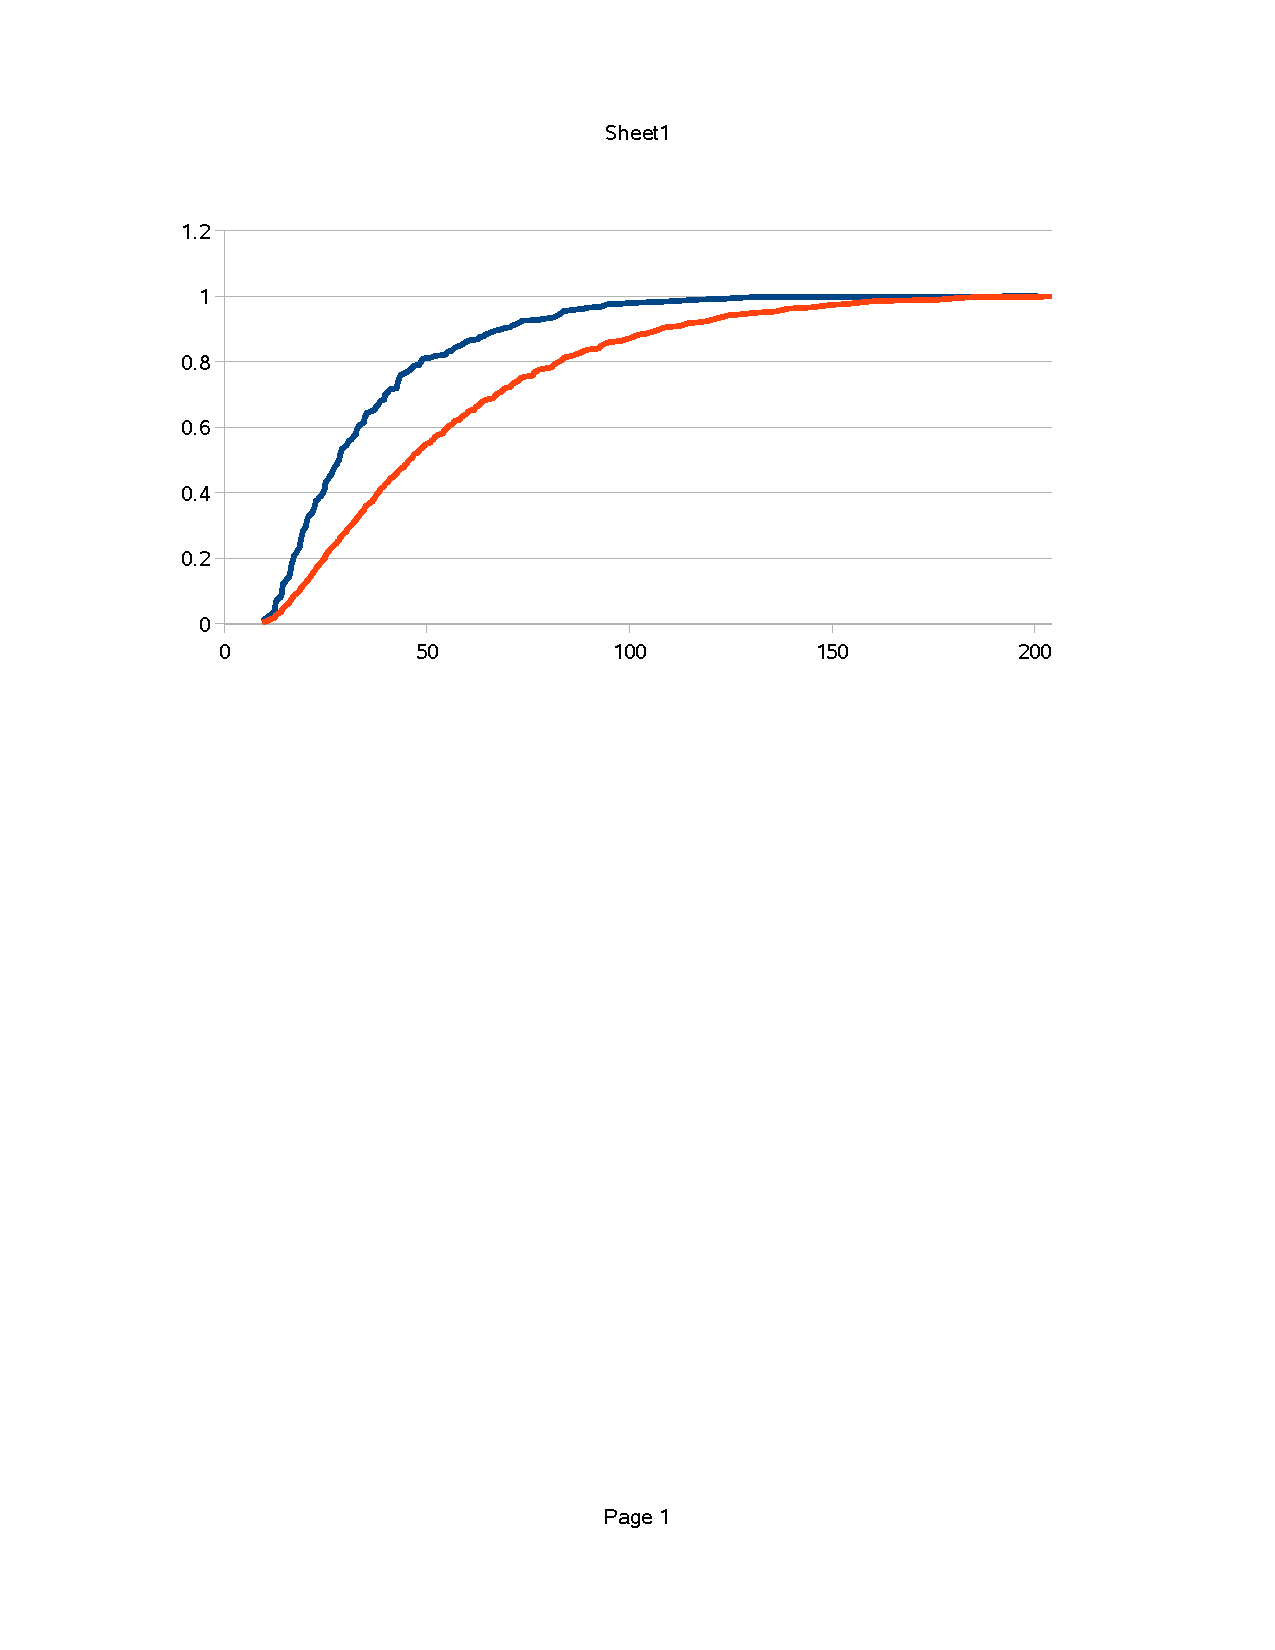
\includepdf[pages={1}]{KS.pdf}
  	
\end{document}
